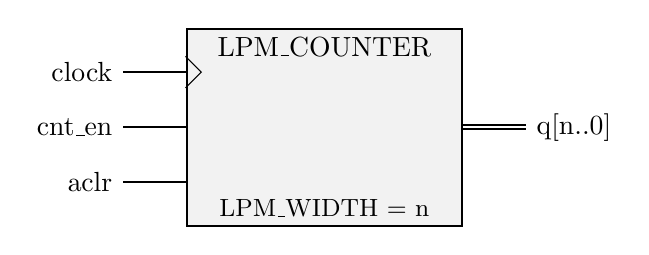
\begin{tikzpicture}
    % LPM Block
    \node [draw, minimum width=3.5cm, minimum height=2.5cm, thick, fill=lightgray!20] (lpm) {};
    
    % Label
    \node [anchor=north] at (lpm.north) {LPM\_COUNTER};
    
    % Inputs
    \draw [thick] (lpm.west) ++(0, 0.7) coordinate (clk_in) -- ++(-0.8, 0) node[anchor=east] {clock};
    \draw (lpm.west) ++(0, 0.5) -- ++(0.2, 0.2) -- ++(-0.2, 0.2); % Clock triangle
    
    \draw [thick] (lpm.west) ++(0, 0) coordinate (cnt_en) -- ++(-0.8, 0) node[anchor=east] {cnt\_en};
    
    \draw [thick] (lpm.west) ++(0, -0.7) coordinate (aclr) -- ++(-0.8, 0) node[anchor=east] {aclr};
    
    % Outputs
    \draw [thick, double] (lpm.east) ++(0, 0) coordinate (q_out) -- ++(0.8, 0) node[anchor=west] {q[n..0]};
    
    % Parameters (Visual representation)
    \node [anchor=south] at (lpm.south) {\small LPM\_WIDTH = n};
\end{tikzpicture}
